% !TEX options=--shell-escape --file-line-error --interaction=nonstopmode %DOCFILE%
% !TEX program=xelatex
\documentclass[frontonly]{poker}

\iffontspecavali
\setmainfont{STIX}
\setmonofont{NewComputerModernMono10}
\setsansfont{NewComputerModernSans10}
\fi


\psetup{
  % hoffset=10mm,
  % topoffset=8.5mm,
  poker box style={fit fontsize macros},
  poker auto load file=false,
  poker curr file={},
  poker font name={cmunrb.otf},
}

\def\picname{./Leonhard_Euler.png}

\NewDocumentCommand\fibonaccispiral{O{0.05}O{}m}{
  \ifnum\numexpr#3>0
    % \draw [help lines] (0,0) rectangle ++(#1,-#1);
    \begin{scope}[shift={(#1,-#1)},rotate=-90,scale=1.6180339887]
      \fibonaccispiral[#1][#2]{#3-1}
    \end{scope}
    \path [draw=darkgolden,line width=.3pt,#2] (0,0) arc (90:0:#1);
  \fi
}

\pcolorlet{pokerback}{black}
\pcolorlet{pokerfront}{black}
\colorlet{pokerblk}{-.!50!black}
\pcolorlet{pokercolorc}{pokerblk}
\pcolorlet{pokercolors}{pokerblk}

% \usetikzlibrary{external}
% \tikzexternalize[
%   prefix=tikz-external/,
%   optimize=false,force remake,
% ]

\begin{document}


% \pokerpagebox(1)[poker show main grid,poker show pos]{}


% \begin{pokerpage}(1)[poker show main grid,poker show pos]
% % \begin{scope}[shift=(poker center)]
% % \end{scope}
% \end{pokerpage}

% \pokerpagebox[poker name=1-]{}
% \pokerpagebox[poker index=1]{}
% \pokerpagebox[poker index=54]{}


% \def\tdrawpicture#1{\path[fill overzoom image={#1},draw=red] (poker top golden) circle (10mm and 16mm);}
% \pmaplist*{\namelist}{\pokerpagebox(1)[poker show main grid,poker show pos]{\tdrawpicture{#1}}}
% \pokerpagebox(1)[poker show main grid,poker show pos]{}

\begin{pokerfront}(1)
\coordinate (picture center) at (poker top golden);
% \path[fill overzoom image={Leonhard_Euler.png},draw=red] (picture center) circle (10mm and 16mm);
% \node at (picture center) {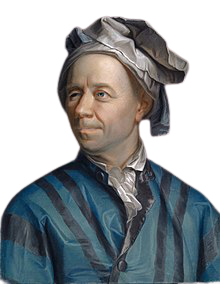
\includegraphics{Leonhard_Euler.png}};
\pimagebox{\paperwidth-13mm,\paperheight-13mm}{(6.5mm,6.5mm)}{\picname}{}
\pshowpos\pshowgrid[thin,opacity=.4]
\end{pokerfront}

\begin{pokerfront}(2)[poker topoffset=8.5mm]
\pimagebox[node={anchor=center,name=portrait}]{30mm,36mm}{([yshift=4mm]poker top golden)}{\picname}{}
% \node [at=(image.north),anchor=south,draw=blue] {Leonhard Euler};
\ptopbox[empty,boxrule=1pt,no inner space,halign=center,valign=bottom,colupper=pokertextcolor,fontupper=\Large]{Leonhard Euler}
\pnodebox[name=accomplishment]{(poker bot golden)}{\sffamily\bfseries\LARGE Euler Formula}
\pnodebox[name=details,anchor=north]{([yshift=-1mm]accomplishment.south)}{\Huge $\mathrm{e}\sp{\mathrm{i}\uppi}+1=0$}
\pnodebox[name=infomation,anchor=north]{([yshift=-3mm]details.south)}
  {\begin{minipage}{\dimexpr\paperwidth-20mm}
    \centering
    The most famous mathematician in 19 century
   \end{minipage}}
\pshowpos\pshowgrid[thin,opacity=.4]
\end{pokerfront}

\begin{pokerback}[poker show main grid={very thin,opacity=.4}]
\begin{scope}[color=pokermathcolor,very thin,shift=(poker center)]
\foreach \i in {15mm,20mm,25mm,30mm,35mm,40mm,45mm,50mm} \draw[line width=.3pt] (0,0) circle (\i);
\foreach \r in {0,18,...,359} {
  \draw[rotate=\r] plot [domain=0:1.5] ({\x*cos(\x r)},{\x*sin(\x r)});
  \draw[rotate=\r] plot [domain=0:1.5] ({\x*sin(\x r)},{\x*cos(\x r)});}
\fibonaccispiral[0.044]{8}
\draw[clip] plot[domain=0:4.76*pi,samples=600] ({.1*\x*cos(\x r)},{.1*\x*sin(\x r)});
\end{scope}
\end{pokerback}

\begin{pokerfront}[poker topoffset=8.5mm]
\pimagebox[node={anchor=center,name=portrait}]{30mm,36mm}{([yshift=1mm]poker top golden)}{\picname}{}
% \node [at=(image.north),anchor=south,draw=blue] {Leonhard Euler};
\ptopbox[empty,boxrule=1pt,no inner space,halign=center,valign=bottom,colupper=pokertextcolor,fontupper=\Large]{Leonhard Euler}
\pnodebox[name=accomplishment]{([yshift=-3mm]poker bot golden)}{\sffamily\bfseries\LARGE Euler Formula}
\pnodebox[name=details,anchor=north]{([yshift=-1mm]accomplishment.south)}{\Huge $\mathrm{e}\sp{\mathrm{i}\uppi}+1=0$}
\pnodebox[name=infomation,anchor=north]{([yshift=-3mm]details.south)}
  {\begin{minipage}{\dimexpr\paperwidth-20mm}
    \centering
    The most famous mathematician in 19 century
   \end{minipage}}
%\pshowpos\pshowgrid[thin,opacity=.4]
\end{pokerfront}

\clearpage

% predefined color
\pcolorlet{pokerback}{white}
\pcolorlet{pokerfront}{white}
\pcolorlet{pokerblk}{black}
\pcolorlet{pokercolorc}{pokerblk}
\pcolorlet{pokercolors}{pokerblk}
\pcolorlet{pokertextcolor}{red!50!black}
\pcolorlet{pokermathcolor}{red!50!black}

%% define color
\pcolorlet{ddarkred}{red!50!black}

\begin{pokerfront}(1)
\coordinate (picture center) at (poker top golden);
% \path[fill overzoom image={Leonhard_Euler.png},draw=red] (picture center) circle (10mm and 16mm);
% \node at (picture center) {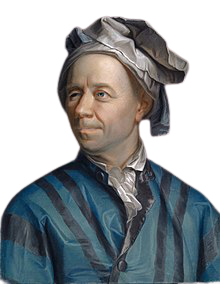
\includegraphics{Leonhard_Euler.png}};
\pimagebox{\paperwidth-13mm,\paperheight-13mm}{(6.5mm,6.5mm)}{\picname}{}
% \pshowpos\pshowgrid[thin,opacity=.4]
\end{pokerfront}

\begin{pokerfront}(2)[poker topoffset=8.5mm]
\pimagebox[node={anchor=center,name=portrait}]{30mm,36mm}{([yshift=4mm]poker top golden)}{\picname}{}
% \node [at=(image.north),anchor=south,draw=blue] {Leonhard Euler};
\ptopbox[empty,boxrule=1pt,no inner space,halign=center,valign=bottom,colupper=pokertextcolor,fontupper=\Large]{Leonhard Euler}
\pnodebox[name=accomplishment, color=ddarkred]{(poker bot golden)}{\sffamily\bfseries\LARGE Euler Formula}
\pnodebox[name=details,anchor=north, color=ddarkred]{([yshift=-1mm]accomplishment.south)}{\Huge $\mathrm{e}\sp{\mathrm{i}\uppi}+1=0$}
\pnodebox[name=infomation,anchor=north]{([yshift=-3mm]details.south)}
  {\begin{minipage}{\dimexpr\paperwidth-20mm}
    \centering\color{ddarkred}
    The most famous mathematician in 19 century
   \end{minipage}}
% \pshowpos\pshowgrid[thin,opacity=.4]
\end{pokerfront}

\begin{pokerback}[poker show main grid={very thin,opacity=.4}]
\begin{scope}[color=pokermathcolor,very thin,shift=(poker center)]
\foreach \i in {15mm,20mm,25mm,30mm,35mm,40mm,45mm,50mm} \draw[line width=.3pt] (0,0) circle (\i);
\foreach \r in {0,18,...,359} {
  \draw[rotate=\r] plot [domain=0:1.5] ({\x*cos(\x r)},{\x*sin(\x r)});
  \draw[rotate=\r] plot [domain=0:1.5] ({\x*sin(\x r)},{\x*cos(\x r)});}
\fibonaccispiral[0.044][color=ddarkred]{8}
\draw[clip] plot[domain=0:4.76*pi,samples=600] ({.1*\x*cos(\x r)},{.1*\x*sin(\x r)});
\end{scope}
\end{pokerback}


\begin{pokerfront}[poker topoffset=8.5mm]
\pimagebox[node={anchor=center,name=portrait}]{30mm,36mm}{([yshift=1mm]poker top golden)}{\picname}{}
% \node [at=(image.north),anchor=south,draw=blue] {Leonhard Euler};
\ptopbox[empty,boxrule=1pt,no inner space,halign=center,valign=bottom,colupper=pokertextcolor,fontupper=\Large]{Leonhard Euler}
\pnodebox[name=accomplishment, color=ddarkred]{([yshift=-3mm]poker bot golden)}{\sffamily\bfseries\LARGE Euler Formula}
\pnodebox[name=details,anchor=north, color=ddarkred]{([yshift=-1mm]accomplishment.south)}{\Huge $\mathrm{e}\sp{\mathrm{i}\uppi}+1=0$}
\pnodebox[name=infomation,anchor=north]{([yshift=-3mm]details.south)}
  {\begin{minipage}{\dimexpr\paperwidth-20mm}
    \centering\color{ddarkred}
    The most famous mathematician in 19 century
   \end{minipage}}
% \pshowpos\pshowgrid[thin,opacity=.4]
\end{pokerfront}

% \pmaplist*{\namelist}{\pokerpagebox(1)[poker show main grid,poker show pos]{\tdrawpicture{#1}}}


\end{document}